\apendice{Especificación de Requisitos}

\section{Introducción}
Este apartado consistirá en una descripción de los propósitos y requerimientos de la aplicación.

\section{Objetivos generales}
El objetivo principal del proyecto es el crear una aplicación web, esta debe tener control de usuarios y capacidad de clasificar imágenes mediante una red neuronal. Por último debe ser capaz de re-entrenar el modelo de clasificación de imágenes.

La red neuronal a usar es inception v3 y el conjunto de datos es Imagenet.

Además se pide que todo esto se haga de una manera escalable, desplegable y con un enfoque que reduzca la deuda técnica.

\section{Catalogo de requisitos}
\subsection{Requisitos funcionales}
\begin{itemize}
\tightlist
\item
  \textbf{RF-1 Control de usuarios:} la aplicación tiene que tener capacidades para controlar usuarios.

  \begin{itemize}
  \tightlist
  \item
    \textbf{RF-1.1 Registro de usuarios:} el usuario debe poder registrarse en la aplicación con su correo.
  \item
    \textbf{RF-1.2 Login:} el usuario debe poder entrar a la aplicación una vez esté registrado.
  \item
    \textbf{RF-1.3 Logout:} el usuario debe poder finalizar una sesión.
  \item
    \textbf{RF-1.4 Integración con Google:} en caso de que el usuario tenga cuenta de google podrá usarla para hacer el login.
  \end{itemize}
\item
  \textbf{RF-2 Uso de aprendizaje automático:} se debe permitir el uso de un sistema de aprendizaje automático basado en una red neuronal.
  
  \begin{itemize}
  \tightlist
  \item
    \textbf{RF-2.1 Clasificación de imágenes:} el usuario podrá clasificar imágenes individuales.
  \item
    \textbf{RF-2.2 Re-entrenamiento del modelo:} se deberá permitir el re-entrenamiento de la red neuronal con distintos conjuntos de datos.
    
  \end{itemize}
\item
  \textbf{RF-3 Manejo de imágenes:} el usuario podrá subir imágenes para ser usadas por los algoritmos de aprendizaje automático.
  
  \begin{itemize}
  \tightlist
  \item
    \textbf{RF-3.1 Subir imagen individual:} se necesita poder subir imágenes individuales para su posterior clasificación.
  \item
    \textbf{RF-3.2 Subir conjunto de imágenes:} se podrá subir un conjunto de imágenes con un formato determinado para poder re-entrenar los modelos.    
  \end{itemize}
\end{itemize}

\subsection{Requisitos no funcionales}

\begin{itemize}
\tightlist
\item
  \textbf{RNF-1 Usabilidad:} la aplicación debe ser intuitiva y con una interfaz sencilla.
\item
  \textbf{RNF-2 Responsividad:} la interfaz tiene que cambiar de tamaño y dimensiones con respecto a la pantalla y su tamaño.
\item
  \textbf{RNF-3 Escalabilidad:} la aplicación debe poder aumentar su rendimiento con el incremento de recursos hardware.
\item
  \textbf{RNF-4 Seguridad:} Los datos sensibles, como las contraseñas, deben tratarse de forma segura. También se tendrá que tener las medidas básicas de seguridad contra los ataques a web más comunes.
\item
  \textbf{RNF-5 Mantenibilidad}: la aplicación debe ser desarrollada de manera que permita escalabilidad a la hora de añadir características. 
\item
  \textbf{RNF-6 Internacionalización}: la aplicación deberá estar preparada para soportar varios idiomas.
\item
  \textbf{RNF-7 Facilidad de despliegue:} se debe poder desplegar la aplicación en poco tiempo.
\end{itemize}

\section{Especificación de requisitos}
En esta sección se desarrollarán los casos de uso de la aplicación, cabe destacar que los actores del sistema corresponden a la misma persona en distintos momentos de su uso de la aplicación.

\begin{figure}
	\centering
	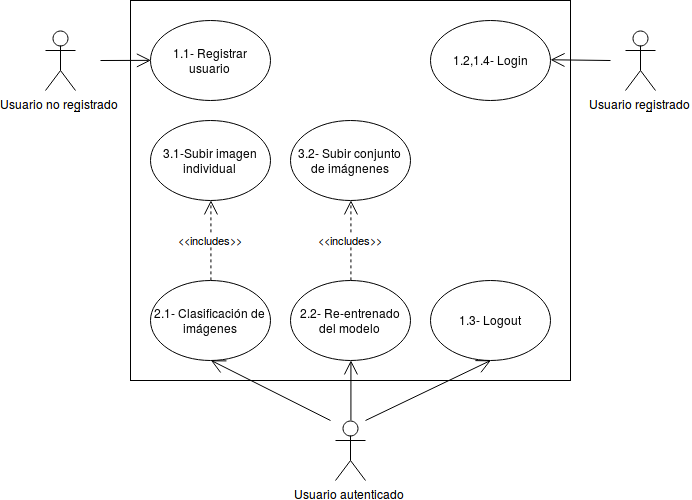
\includegraphics[width=0.8\textwidth]{usecase.png}
	\caption{Diagrama de casos de uso}\label{fig:usecase.png}
\end{figure}



\begin{longtable}[H]{@{}ll@{}}
\toprule
\begin{minipage}[b]{0.26\columnwidth}\raggedright\strut%-----------------------------------------------------------------------
\textbf{CU-01}\strut
\end{minipage} & \begin{minipage}[b]{0.68\columnwidth}\raggedright\strut%-----------------------------------------------------------------------
\textbf{Registro de usuario}\strut
\end{minipage}\tabularnewline
\midrule
\endhead
\begin{minipage}[t]{0.26\columnwidth}\raggedright\strut
\textbf{Autor}\strut
\end{minipage} & \begin{minipage}[t]{0.68\columnwidth}\raggedright\strut
Javier Martínez Riberas\strut
\end{minipage}\tabularnewline
\begin{minipage}[t]{0.26\columnwidth}\raggedright\strut
\textbf{Requisitos asociados}\strut
\end{minipage} & \begin{minipage}[t]{0.68\columnwidth}\raggedright\strut%-----------------------------------------------------------------------
RF-1.1\strut
\end{minipage}\tabularnewline
\begin{minipage}[t]{0.26\columnwidth}\raggedright\strut
\textbf{Descripción}\strut
\end{minipage} & \begin{minipage}[t]{0.68\columnwidth}\raggedright\strut%-----------------------------------------------------------------------
Permite al usuario registrarse.\strut
\end{minipage}\tabularnewline
\begin{minipage}[t]{0.26\columnwidth}\raggedright\strut
\textbf{Precondición}\strut
\end{minipage} & \begin{minipage}[t]{0.68\columnwidth}\raggedright\strut%-----------------------------------------------------------------------
Ninguna.\strut
\end{minipage}\tabularnewline
\begin{minipage}[t]{0.26\columnwidth}\raggedright\strut
\textbf{Acciones}\strut
\end{minipage} & \begin{minipage}[t]{0.68\columnwidth}\raggedright\strut%-----------------------------------------------------------------------
\begin{enumerate}
\def\labelenumi{\arabic{enumi}.}
\tightlist
\item
  El usuario rellena el formulario de registro (email y contraseña).
\item
  Si esta configurada la confirmación por email se necesita confirmar para terminar el registro.
\end{enumerate}\strut
\end{minipage}\tabularnewline
\begin{minipage}[t]{0.26\columnwidth}\raggedright\strut
\textbf{Postcondición}\strut
\end{minipage} & \begin{minipage}[t]{0.68\columnwidth}\raggedright\strut%-----------------------------------------------------------------------
El usuario se registra en la base de datos.\strut
\end{minipage}\tabularnewline
\begin{minipage}[t]{0.26\columnwidth}\raggedright\strut
\textbf{Excepciones}\strut
\end{minipage} & \begin{minipage}[t]{0.68\columnwidth}\raggedright\strut%-----------------------------------------------------------------------
\begin{itemize}
\tightlist
\item
  Fallo de la configuración de email. (Si no hay no se da)
\end{itemize}\strut
\end{minipage}\tabularnewline
\begin{minipage}[t]{0.26\columnwidth}\raggedright\strut
\textbf{Importancia}\strut
\end{minipage} & \begin{minipage}[t]{0.68\columnwidth}\raggedright\strut%-----------------------------------------------------------------------
Alta\strut
\end{minipage}\tabularnewline
\bottomrule%------------------------------------------------------------
\caption{CU-01 Registro de usuario.}
\end{longtable}

%------------------------------------------------------------------------------------------

\begin{longtable}[H]{@{}ll@{}}
\toprule
\begin{minipage}[b]{0.26\columnwidth}\raggedright\strut%-----------------------------------------------------------------------
\textbf{CU-02}\strut
\end{minipage} & \begin{minipage}[b]{0.68\columnwidth}\raggedright\strut%-----------------------------------------------------------------------
\textbf{Login}\strut
\end{minipage}\tabularnewline
\midrule
\endhead
\begin{minipage}[t]{0.26\columnwidth}\raggedright\strut
\textbf{Autor}\strut
\end{minipage} & \begin{minipage}[t]{0.68\columnwidth}\raggedright\strut
Javier Martínez Riberas\strut
\end{minipage}\tabularnewline
\begin{minipage}[t]{0.26\columnwidth}\raggedright\strut
\textbf{Requisitos asociados}\strut
\end{minipage} & \begin{minipage}[t]{0.68\columnwidth}\raggedright\strut%-----------------------------------------------------------------------
RF-1.2, RF-1.4\strut
\end{minipage}\tabularnewline
\begin{minipage}[t]{0.26\columnwidth}\raggedright\strut
\textbf{Descripción}\strut
\end{minipage} & \begin{minipage}[t]{0.68\columnwidth}\raggedright\strut%-----------------------------------------------------------------------
Permite al usuario autenticarse.\strut
\end{minipage}\tabularnewline
\begin{minipage}[t]{0.26\columnwidth}\raggedright\strut
\textbf{Precondición}\strut
\end{minipage} & \begin{minipage}[t]{0.68\columnwidth}\raggedright\strut%-----------------------------------------------------------------------
El usuario debe de estar registrado.\strut
\end{minipage}\tabularnewline
\begin{minipage}[t]{0.26\columnwidth}\raggedright\strut
\textbf{Acciones}\strut
\end{minipage} & \begin{minipage}[t]{0.68\columnwidth}\raggedright\strut%-----------------------------------------------------------------------
\begin{enumerate}
\def\labelenumi{\arabic{enumi}.}
\tightlist
\item
  El usuario rellena el formulario de login (email y contraseña). O el equivalente en google.
\end{enumerate}\strut
\end{minipage}\tabularnewline
\begin{minipage}[t]{0.26\columnwidth}\raggedright\strut
\textbf{Postcondición}\strut
\end{minipage} & \begin{minipage}[t]{0.68\columnwidth}\raggedright\strut%-----------------------------------------------------------------------
El usuario consigue una sesión.\strut
\end{minipage}\tabularnewline
\begin{minipage}[t]{0.26\columnwidth}\raggedright\strut
\textbf{Excepciones}\strut
\end{minipage} & \begin{minipage}[t]{0.68\columnwidth}\raggedright\strut%-----------------------------------------------------------------------
\begin{itemize}
\tightlist
\item
  Fallo de rellenado del formulario.
\end{itemize}\strut
\end{minipage}\tabularnewline
\begin{minipage}[t]{0.26\columnwidth}\raggedright\strut
\textbf{Importancia}\strut
\end{minipage} & \begin{minipage}[t]{0.68\columnwidth}\raggedright\strut%-----------------------------------------------------------------------
Alta\strut
\end{minipage}\tabularnewline
\bottomrule%------------------------------------------------------------
\caption{CU-02 Login.}
\end{longtable}

%------------------------------------------------------------------------------------------

\begin{longtable}[H]{@{}ll@{}}
\toprule
\begin{minipage}[b]{0.26\columnwidth}\raggedright\strut%-----------------------------------------------------------------------
\textbf{CU-03}\strut
\end{minipage} & \begin{minipage}[b]{0.68\columnwidth}\raggedright\strut%-----------------------------------------------------------------------
\textbf{Logout}\strut
\end{minipage}\tabularnewline
\midrule
\endhead
\begin{minipage}[t]{0.26\columnwidth}\raggedright\strut
\textbf{Autor}\strut
\end{minipage} & \begin{minipage}[t]{0.68\columnwidth}\raggedright\strut
Javier Martínez Riberas\strut
\end{minipage}\tabularnewline
\begin{minipage}[t]{0.26\columnwidth}\raggedright\strut
\textbf{Requisitos asociados}\strut
\end{minipage} & \begin{minipage}[t]{0.68\columnwidth}\raggedright\strut%-----------------------------------------------------------------------
RF-1.3\strut
\end{minipage}\tabularnewline
\begin{minipage}[t]{0.26\columnwidth}\raggedright\strut
\textbf{Descripción}\strut
\end{minipage} & \begin{minipage}[t]{0.68\columnwidth}\raggedright\strut%-----------------------------------------------------------------------
El usuario se des-autentica.\strut
\end{minipage}\tabularnewline
\begin{minipage}[t]{0.26\columnwidth}\raggedright\strut
\textbf{Precondición}\strut
\end{minipage} & \begin{minipage}[t]{0.68\columnwidth}\raggedright\strut%-----------------------------------------------------------------------
El usuario debe de estar autenticado.\strut
\end{minipage}\tabularnewline
\begin{minipage}[t]{0.26\columnwidth}\raggedright\strut
\textbf{Acciones}\strut
\end{minipage} & \begin{minipage}[t]{0.68\columnwidth}\raggedright\strut%-----------------------------------------------------------------------
\begin{enumerate}
\def\labelenumi{\arabic{enumi}.}
\tightlist
\item
  El usuario hace click el botón de logout.
\end{enumerate}\strut
\end{minipage}\tabularnewline
\begin{minipage}[t]{0.26\columnwidth}\raggedright\strut
\textbf{Postcondición}\strut
\end{minipage} & \begin{minipage}[t]{0.68\columnwidth}\raggedright\strut%-----------------------------------------------------------------------
El usuario cierra una sesión, la cual se elimina.\strut
\end{minipage}\tabularnewline
\begin{minipage}[t]{0.26\columnwidth}\raggedright\strut
\textbf{Excepciones}\strut
\end{minipage} & \begin{minipage}[t]{0.68\columnwidth}\raggedright\strut%-----------------------------------------------------------------------
Ninguna.\strut
\end{minipage}\tabularnewline
\begin{minipage}[t]{0.26\columnwidth}\raggedright\strut
\textbf{Importancia}\strut
\end{minipage} & \begin{minipage}[t]{0.68\columnwidth}\raggedright\strut%-----------------------------------------------------------------------
Alta\strut
\end{minipage}\tabularnewline
\bottomrule%------------------------------------------------------------
\caption{CU-03 Logout.}
\end{longtable}

%------------------------------------------------------------------------------------------

\begin{longtable}[H]{@{}ll@{}}
\toprule
\begin{minipage}[b]{0.26\columnwidth}\raggedright\strut%-----------------------------------------------------------------------
\textbf{CU-04}\strut
\end{minipage} & \begin{minipage}[b]{0.68\columnwidth}\raggedright\strut%-----------------------------------------------------------------------
\textbf{Clasificar imagen}\strut
\end{minipage}\tabularnewline
\midrule
\endhead
\begin{minipage}[t]{0.26\columnwidth}\raggedright\strut
\textbf{Autor}\strut
\end{minipage} & \begin{minipage}[t]{0.68\columnwidth}\raggedright\strut
Javier Martínez Riberas\strut
\end{minipage}\tabularnewline
\begin{minipage}[t]{0.26\columnwidth}\raggedright\strut
\textbf{Requisitos asociados}\strut
\end{minipage} & \begin{minipage}[t]{0.68\columnwidth}\raggedright\strut%-----------------------------------------------------------------------
RF-2.1, RF-3.1\strut
\end{minipage}\tabularnewline
\begin{minipage}[t]{0.26\columnwidth}\raggedright\strut
\textbf{Descripción}\strut
\end{minipage} & \begin{minipage}[t]{0.68\columnwidth}\raggedright\strut%-----------------------------------------------------------------------
Permite al usuario obtener la clase de una imagen.\strut
\end{minipage}\tabularnewline
\begin{minipage}[t]{0.26\columnwidth}\raggedright\strut
\textbf{Precondición}\strut
\end{minipage} & \begin{minipage}[t]{0.68\columnwidth}\raggedright\strut%-----------------------------------------------------------------------
El usuario debe de estar autenticado.\strut
\end{minipage}\tabularnewline
\begin{minipage}[t]{0.26\columnwidth}\raggedright\strut
\textbf{Acciones}\strut
\end{minipage} & \begin{minipage}[t]{0.68\columnwidth}\raggedright\strut%-----------------------------------------------------------------------
\begin{enumerate}
\def\labelenumi{\arabic{enumi}.}
\tightlist
\item
  El usuario sube una foto.
\item 
  Opcional. El usuario elige un re-entrenamiento específico.
\end{enumerate}\strut
\end{minipage}\tabularnewline
\begin{minipage}[t]{0.26\columnwidth}\raggedright\strut
\textbf{Postcondición}\strut
\end{minipage} & \begin{minipage}[t]{0.68\columnwidth}\raggedright\strut%-----------------------------------------------------------------------
El usuario ve la clase más probable y otras dos probables.\strut
\end{minipage}\tabularnewline
\begin{minipage}[t]{0.26\columnwidth}\raggedright\strut
\textbf{Excepciones}\strut
\end{minipage} & \begin{minipage}[t]{0.68\columnwidth}\raggedright\strut%-----------------------------------------------------------------------
\begin{itemize}
\tightlist
\item
  Fallo de formato de imagen.
\end{itemize}\strut
\end{minipage}\tabularnewline
\begin{minipage}[t]{0.26\columnwidth}\raggedright\strut
\textbf{Importancia}\strut
\end{minipage} & \begin{minipage}[t]{0.68\columnwidth}\raggedright\strut%-----------------------------------------------------------------------
Alta\strut
\end{minipage}\tabularnewline
\bottomrule%------------------------------------------------------------
\caption{CU-04 Clasificación de imagen.}
\end{longtable}

%------------------------------------------------------------------------------------------

\begin{longtable}[H]{@{}ll@{}}
\toprule
\begin{minipage}[b]{0.26\columnwidth}\raggedright\strut%-----------------------------------------------------------------------
\textbf{CU-05}\strut
\end{minipage} & \begin{minipage}[b]{0.68\columnwidth}\raggedright\strut%-----------------------------------------------------------------------
\textbf{Re-entrenado de modelos}\strut
\end{minipage}\tabularnewline
\midrule
\endhead
\begin{minipage}[t]{0.26\columnwidth}\raggedright\strut
\textbf{Autor}\strut
\end{minipage} & \begin{minipage}[t]{0.68\columnwidth}\raggedright\strut
Javier Martínez Riberas\strut
\end{minipage}\tabularnewline
\begin{minipage}[t]{0.26\columnwidth}\raggedright\strut
\textbf{Requisitos asociados}\strut
\end{minipage} & \begin{minipage}[t]{0.68\columnwidth}\raggedright\strut%-----------------------------------------------------------------------
RF-2.2, RF-3.2\strut
\end{minipage}\tabularnewline
\begin{minipage}[t]{0.26\columnwidth}\raggedright\strut
\textbf{Descripción}\strut
\end{minipage} & \begin{minipage}[t]{0.68\columnwidth}\raggedright\strut%-----------------------------------------------------------------------
Permite al usuario re-entrenar la red neuronal.\strut
\end{minipage}\tabularnewline
\begin{minipage}[t]{0.26\columnwidth}\raggedright\strut
\textbf{Precondición}\strut
\end{minipage} & \begin{minipage}[t]{0.68\columnwidth}\raggedright\strut%-----------------------------------------------------------------------
El usuario debe de estar autenticado y haber subido un dataset.\strut
\end{minipage}\tabularnewline
\begin{minipage}[t]{0.26\columnwidth}\raggedright\strut
\textbf{Acciones}\strut
\end{minipage} & \begin{minipage}[t]{0.68\columnwidth}\raggedright\strut%-----------------------------------------------------------------------
\begin{enumerate}
\def\labelenumi{\arabic{enumi}.}
\tightlist
\item
  El usuario elige un dataset.
\item
  El usuario debe esperar una cantidad decente de tiempo y tendrá el modelo disponible.
\end{enumerate}\strut
\end{minipage}\tabularnewline
\begin{minipage}[t]{0.26\columnwidth}\raggedright\strut
\textbf{Postcondición}\strut
\end{minipage} & \begin{minipage}[t]{0.68\columnwidth}\raggedright\strut%-----------------------------------------------------------------------
El usuario tras un periodo de tiempo tiene disponible un modelo.\strut
\end{minipage}\tabularnewline
\begin{minipage}[t]{0.26\columnwidth}\raggedright\strut
\textbf{Excepciones}\strut
\end{minipage} & \begin{minipage}[t]{0.68\columnwidth}\raggedright\strut%-----------------------------------------------------------------------
\begin{itemize}
\tightlist
\item
  Fallo del formato de las imágenes o de la estructura de archivos.
\end{itemize}\strut
\end{minipage}\tabularnewline
\begin{minipage}[t]{0.26\columnwidth}\raggedright\strut
\textbf{Importancia}\strut
\end{minipage} & \begin{minipage}[t]{0.68\columnwidth}\raggedright\strut%-----------------------------------------------------------------------
Media-Alta\strut
\end{minipage}\tabularnewline
\bottomrule%------------------------------------------------------------
\caption{CU-05 Re-entrenado de modelos.}
\end{longtable}